% =====================================================================
% Marco Práctico --- Sección 3.7: Fase 2
% =====================================================================

\subsection{Etapa 2 --- Neuronas Spiking y Sistema Híbrido}
\label{ch:fase2}

En esta segunda fase, el proyecto integra matemáticamente el modelo de neurona biológica Leaky Integrate-and-Fire (LIF) junto con el dispositivo memristivo, creando el primer bloque de construcción analógico (Memristor--Neurona) capaz de emular codificación temporal y procesamiento neuromórfico sensorial.

% =====================================================================
\subsubsection{Etapa 2.1: Neurona LIF y Acoplamiento Híbrido}
\label{sec:etapa2_1}

\paragraph{Implementación Cualitativa y Teoría Física}
El circuito híbrido simulado conecta un modelo de memristor en serie entre un estímulo de entrada (voltaje sensorial o pre-sináptico) y una neurona LIF. El potencial de membrana se representa como el voltaje de un capacitor $V_C(t)$ sujeto a una corriente de fuga paralela $R_{\mathrm{leak}}$; no se trata de un circuito físico medido.

La ecuación diferencial estocástica que rige el potencial de membrana está dada por:
\begin{equation}
C_m \frac{dV_C}{dt} = -\frac{V_C(t) - V_{\mathrm{rest}}}{R_{\mathrm{leak}}} + I_{\mathrm{inj}}(t) + \sigma_n \cdot \eta(t)
\label{eq:lif_hibrida}
\end{equation}

El acoplamiento se logra inyectando la corriente transmembrana $I_{\mathrm{inj}}(t)$, cuyo valor es dictaminado por la ley de Ohm en la rama de entrada a través de la conductancia del memristor dependiente del estado:
\begin{equation}
I_{\mathrm{inj}}(t) = \frac{V_{\mathrm{in}}(t) - V_C(t)}{R_S(x(t))}
\label{eq:i_inyectada}
\end{equation}

Cuando $V_C(t) \geq V_{\mathrm{th}}$, la neurona genera matemáticamente un evento discreto (\textit{spike}), y resetea instantáneamente su potencial a $V_{\mathrm{reset}}$, entrando en un período refractario absoluto.

Para representar un \textit{sensor volátil}, se emplea un modelo computacional inspirado en dióxido de hafnio (HfO$_2$). Incluye un término fenomenológico de relajación del estado en ausencia de estímulo:
\begin{equation}
\frac{dx}{dt} = f(V_M, x) - \frac{x}{\tau_{\mathrm{relax}}} \left(1 - H(V_M - V_{\mathrm{hold}})\right)
\label{eq:hfo2_dinamica}
\end{equation}

Cualitativamente (Figura~\ref{fig:hfo2_isi_hibrido}), en la simulación el estímulo de $1.5\,\mathrm{V}$ cambia el estado y la resistencia del modelo memristivo, modificando la corriente de entrada y los intervalos entre disparos. La figura ilustra adaptación temporal dentro de este modelo; no demuestra transducción biológica ni una respuesta de un dispositivo fabricado.

\begin{figure}[H]
    \centering
    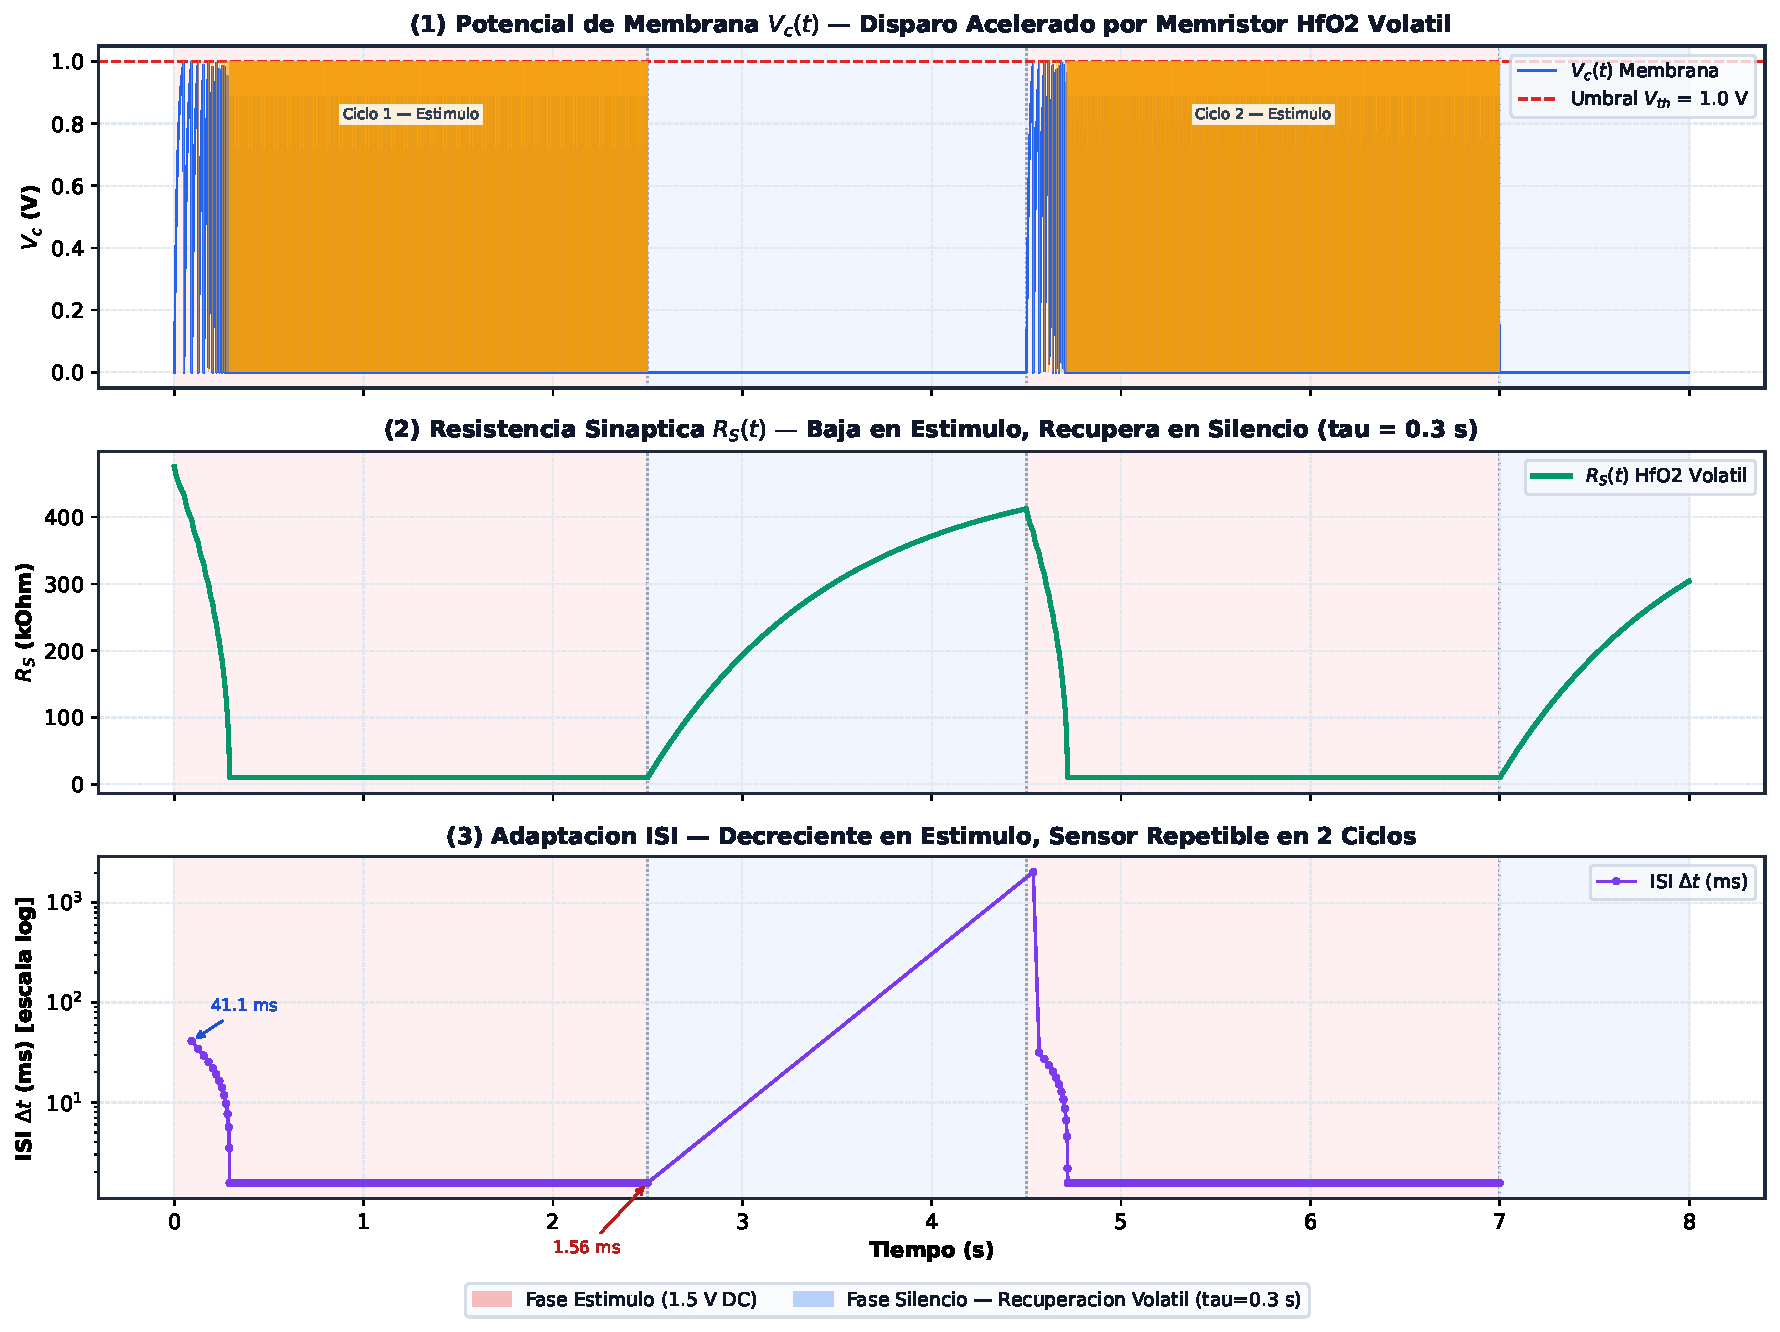
\includegraphics[width=0.85\textwidth]{figuras/fig_06_hfo2_isi_legible.pdf}
    \caption{Respuesta cualitativa del sistema híbrido: Potencial de membrana $V_C(t)$ evidenciando la aceleración temporal (top), Resistencia $R_S(t)$ descendente (centro), e Intervalo Inter-Spike (ISI) modularizado (abajo).}
    \label{fig:hfo2_isi_hibrido}
\end{figure}

\textbf{Propósito y Relevancia:} La figura ilustra el acoplamiento implementado entre el modelo memristivo y la neurona LIF. No constituye una validación de un sensor físico ni de un receptor nociceptivo.

\paragraph{Validación Cuantitativa Computacional}
La integridad matemática de esta fase fue comprobada contra soluciones exactas y papers de referencia del estado del arte.

\begin{figure}[H]
    \centering
    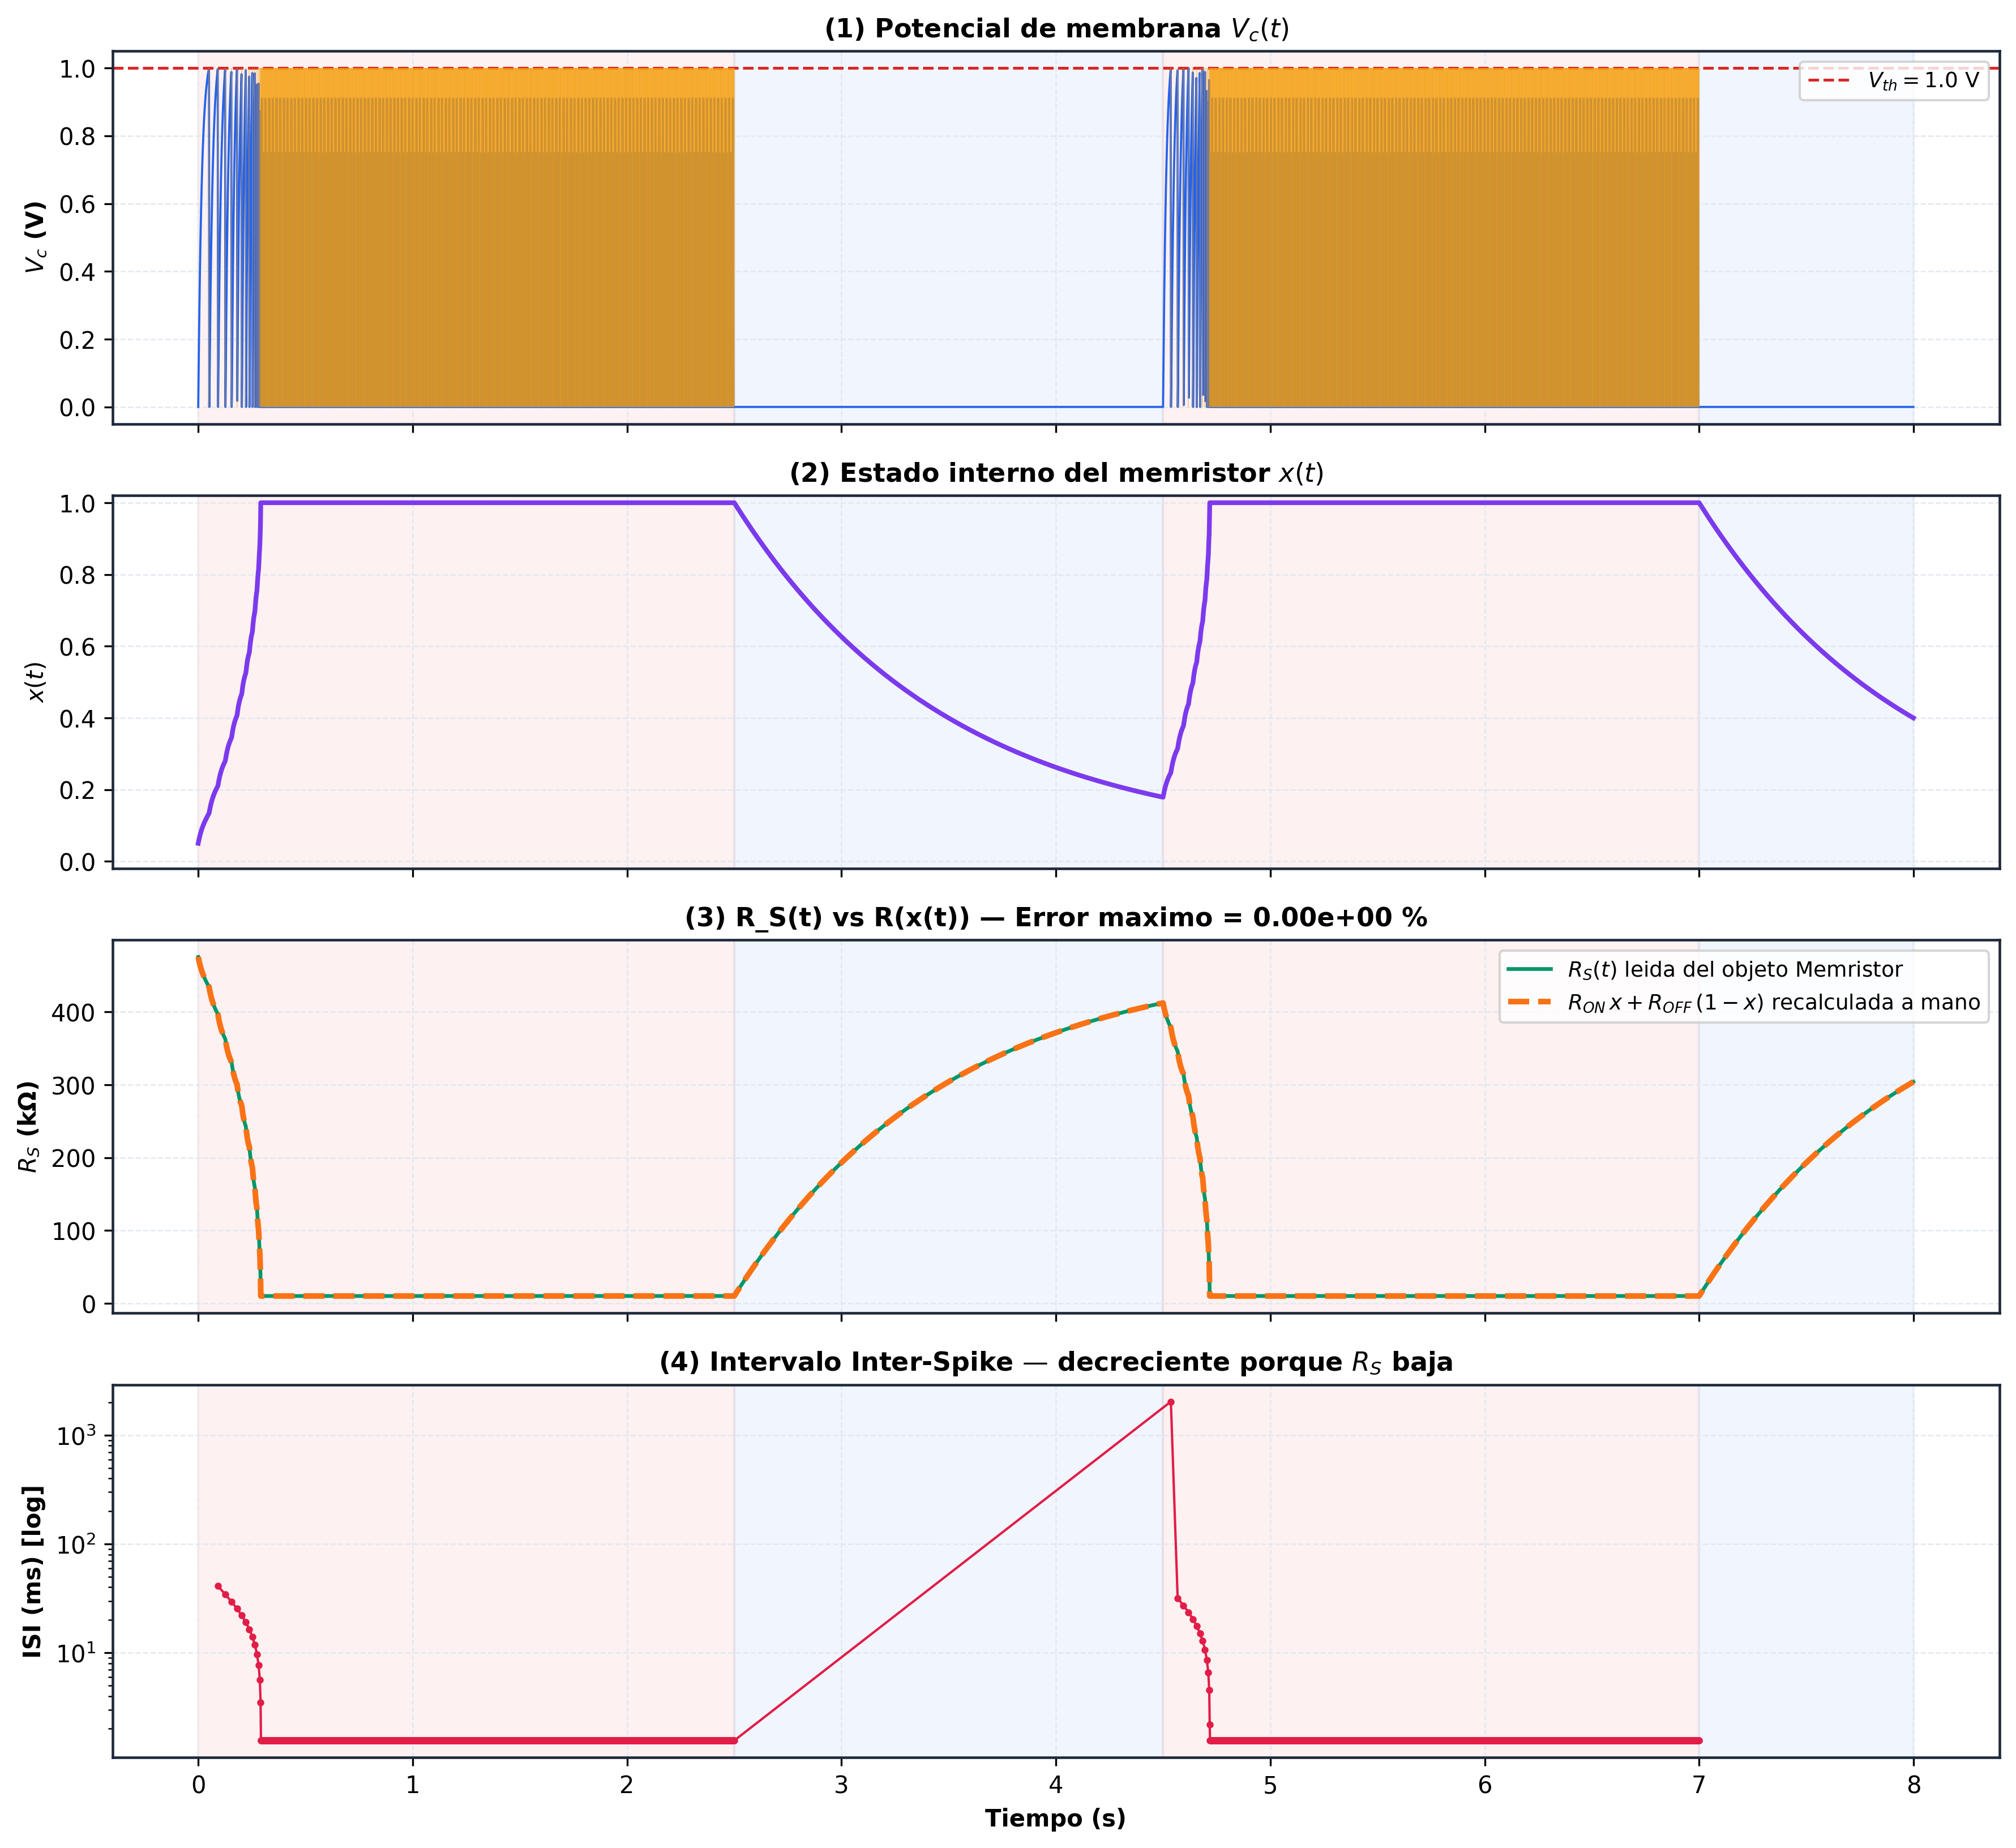
\includegraphics[width=0.7\textwidth]{figuras/fig_08_rs_x.png}
    \caption{Verificación de la resistencia en serie $R_S$ proveniente de la dinámica de acoplamiento de $x$.}
    \label{fig:08_rs_x}
\end{figure}

\textbf{Propósito y Relevancia:} Este gráfico comprueba, para la ejecución y las variables mostradas, la consistencia entre $R_S$ y $x(t)$ según la relación implementada. No prueba por sí solo ausencia general de pérdida de eventos, retrasos ni errores en todas las ejecuciones.

\textbf{Solución Analítica LIF Subumbral:}
Se sometió el módulo integrador numérico de la neurona LIF a una validación estricta frente a su solución analítica exacta de circuito RC subumbral:
\begin{equation}
V_m(t) = V_{\infty} + (V_{m,0} - V_{\infty}) e^{-t/\tau_{eq}}
\end{equation}
La comparación cuantitativa entre la simulación discreta y la solución RC analítica es distinta de la comparación cualitativa con Wang descrita más adelante. En el CSV archivado \texttt{lif\_rc\_validation.csv}, el cálculo de $R^2$ sobre las 1000 muestras disponibles es $0.9999815$, que redondeado a cuatro decimales da $1.0000$. Este resultado describe solo esa prueba subumbral y no se atribuye a la comparación cualitativa ni demuestra exactitud general del integrador para otros pasos o condiciones.

\begin{figure}[H]
    \centering
    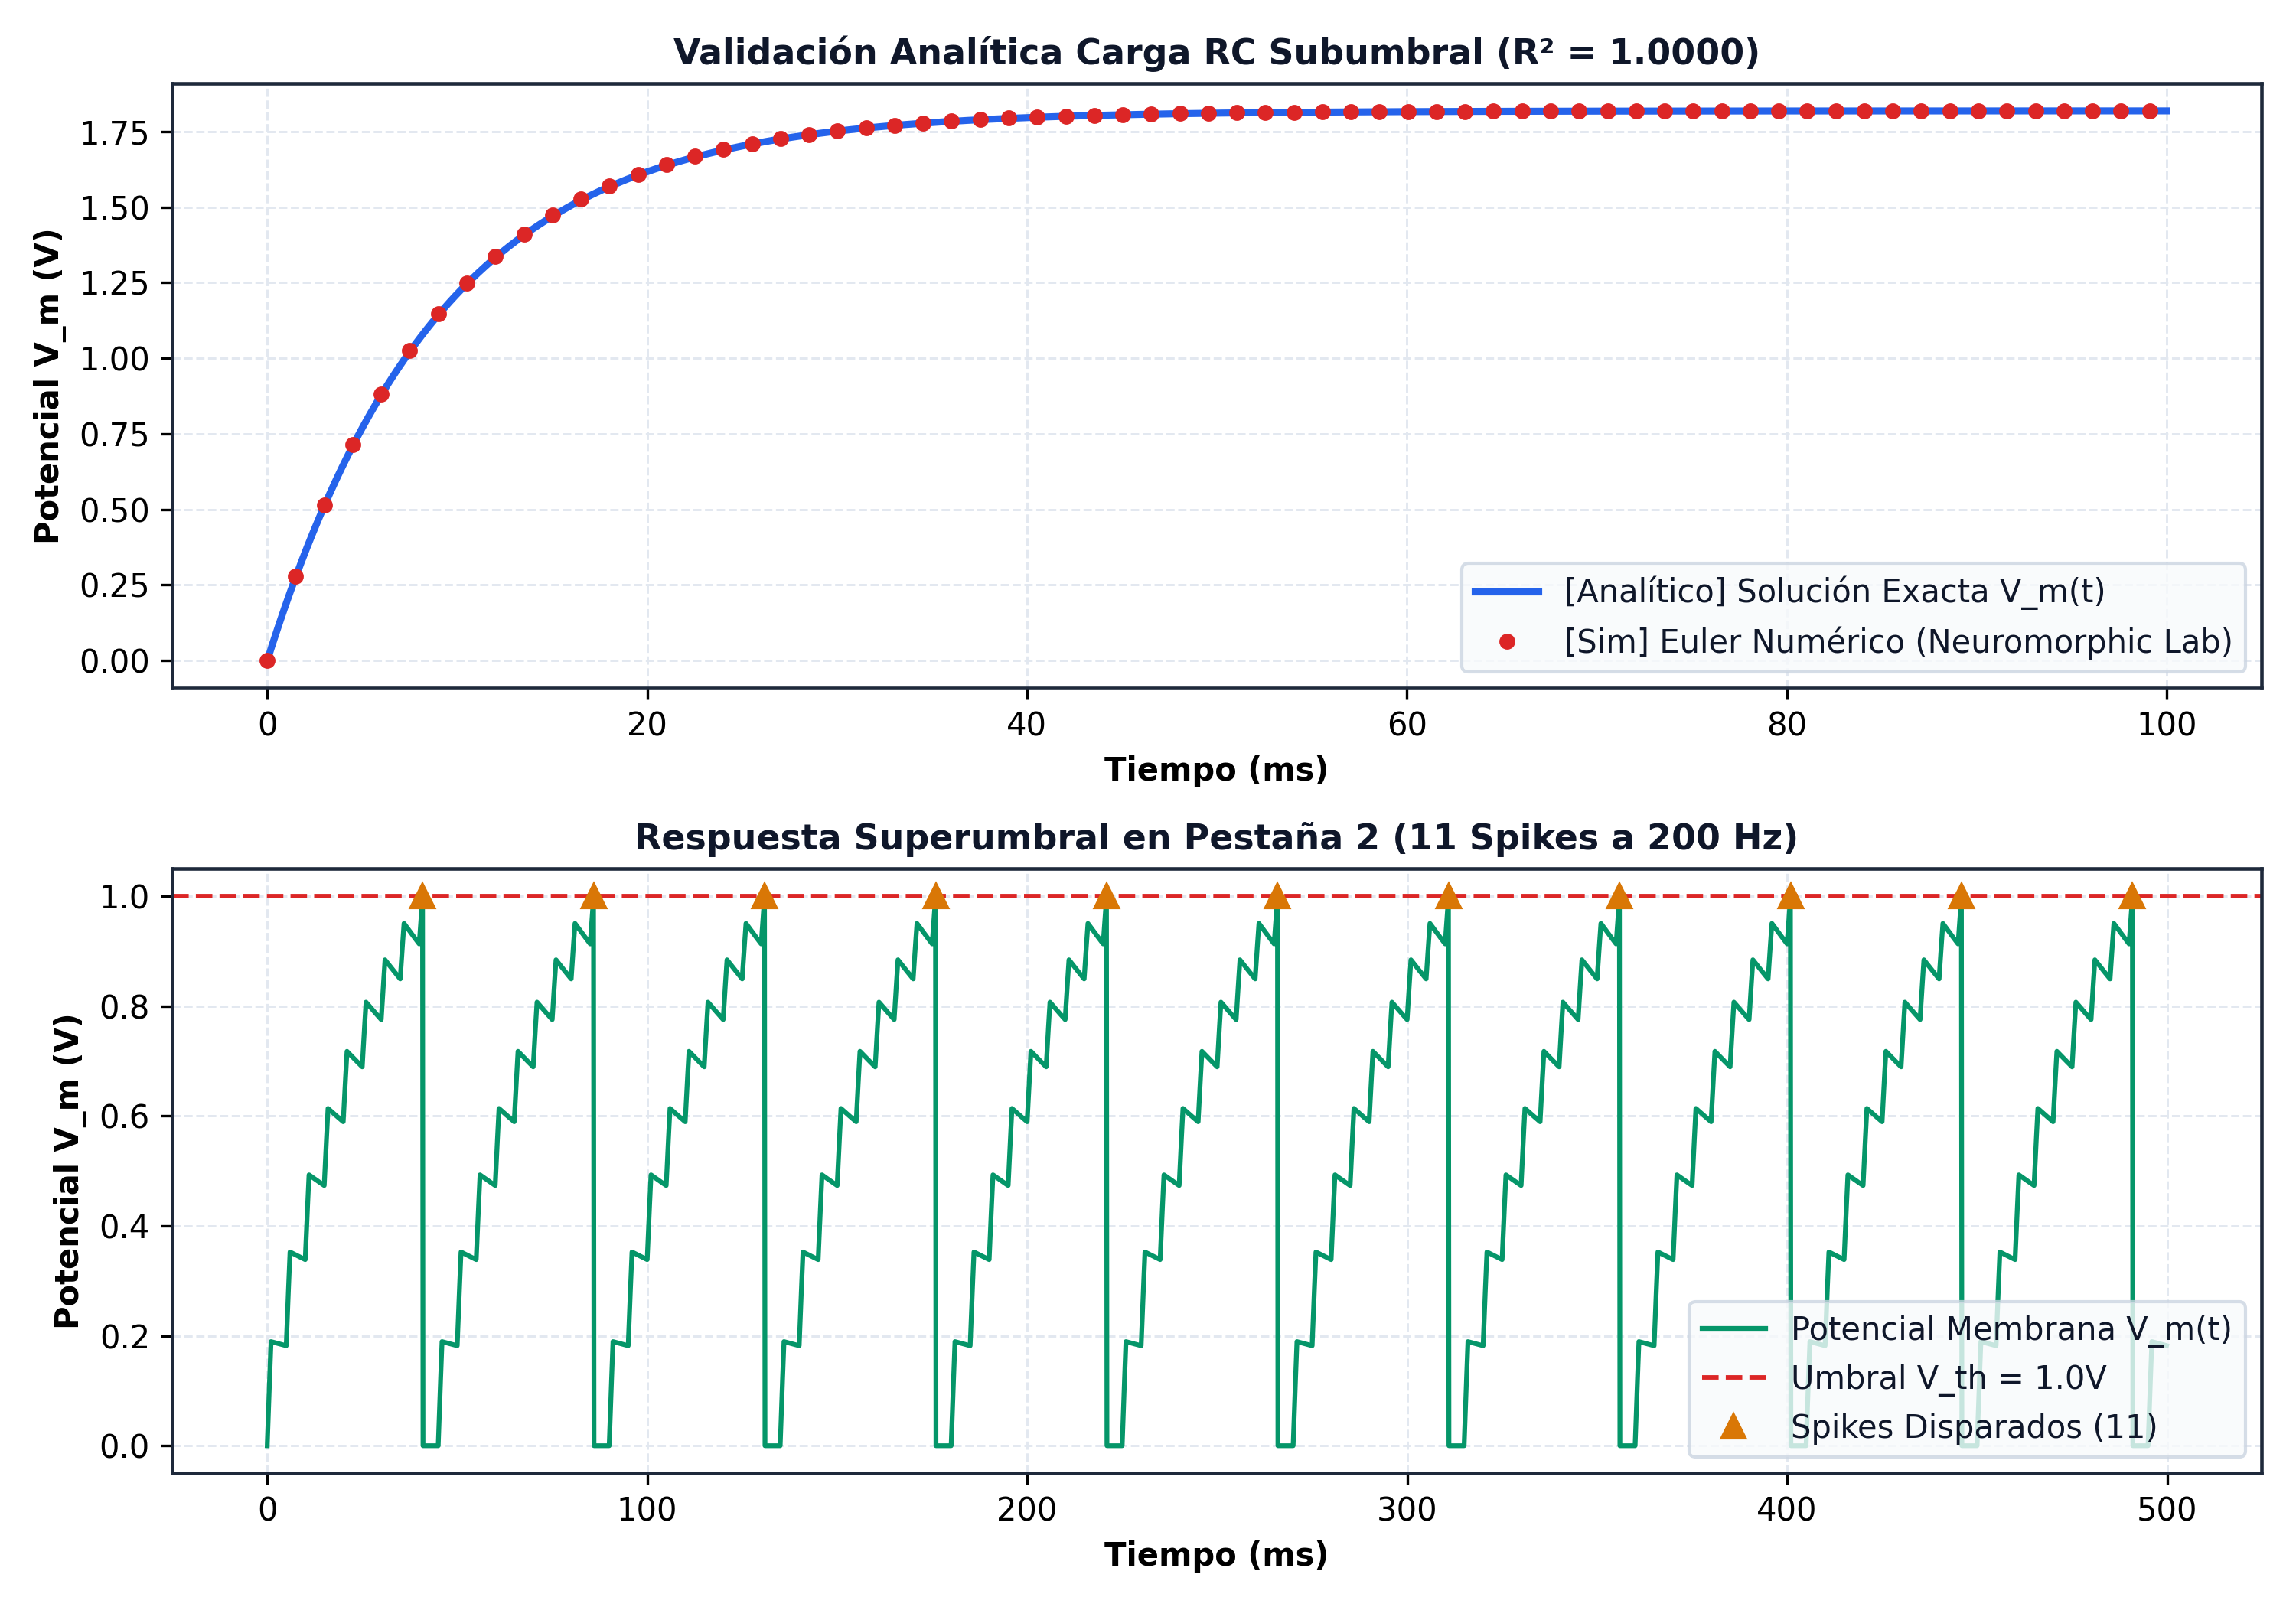
\includegraphics[width=0.85\textwidth]{figuras/fig_03_lif.png}
    \caption{Validación analítica subumbral de la neurona LIF frente a la solución RC exacta en respuesta al impulso.}
    \label{fig:val-lif}
\end{figure}

\textbf{Propósito y Relevancia:} La comparación permite evaluar la respuesta subumbral para las condiciones ensayadas. El valor archivado no basta para descartar sesgos algorítmicos en otras configuraciones ni para afirmar que el núcleo esté libre de errores.

\textbf{Comportamiento cualitativo de integración y disparo LIF:}
La neurona LIF del simulador comparte el comportamiento funcional descrito por Wang et al.~\cite{2}: integra los estímulos, alcanza el umbral y genera eventos de disparo con reinicio. La Figura~\ref{fig:lif-behavior-wang} muestra esta secuencia en el simulador \texttt{Neuromorphic Lab}, con la configuración guardada en \url{02_SOFTWARE/neuromorphic_lab/configs/lif_config.json}: $C_m=100\,\mathrm{nF}$, $R_S=100\,\mathrm{k\Omega}$, $R_{\mathrm{leak}}=1\,\mathrm{M\Omega}$, umbral de $1\,\mathrm{V}$ y período refractario de $2\,\mathrm{ms}$. La entrada simulada es un tren unipolar de $2\,\mathrm{V}$ a $200\,\mathrm{Hz}$, con ciclo útil del $20\%$, durante $0.5\,\mathrm{s}$. Con paso de integración de $1\,\mathrm{\mu s}$, esta ejecución produce 11 eventos de disparo.

\begin{figure}[H]
    \centering
    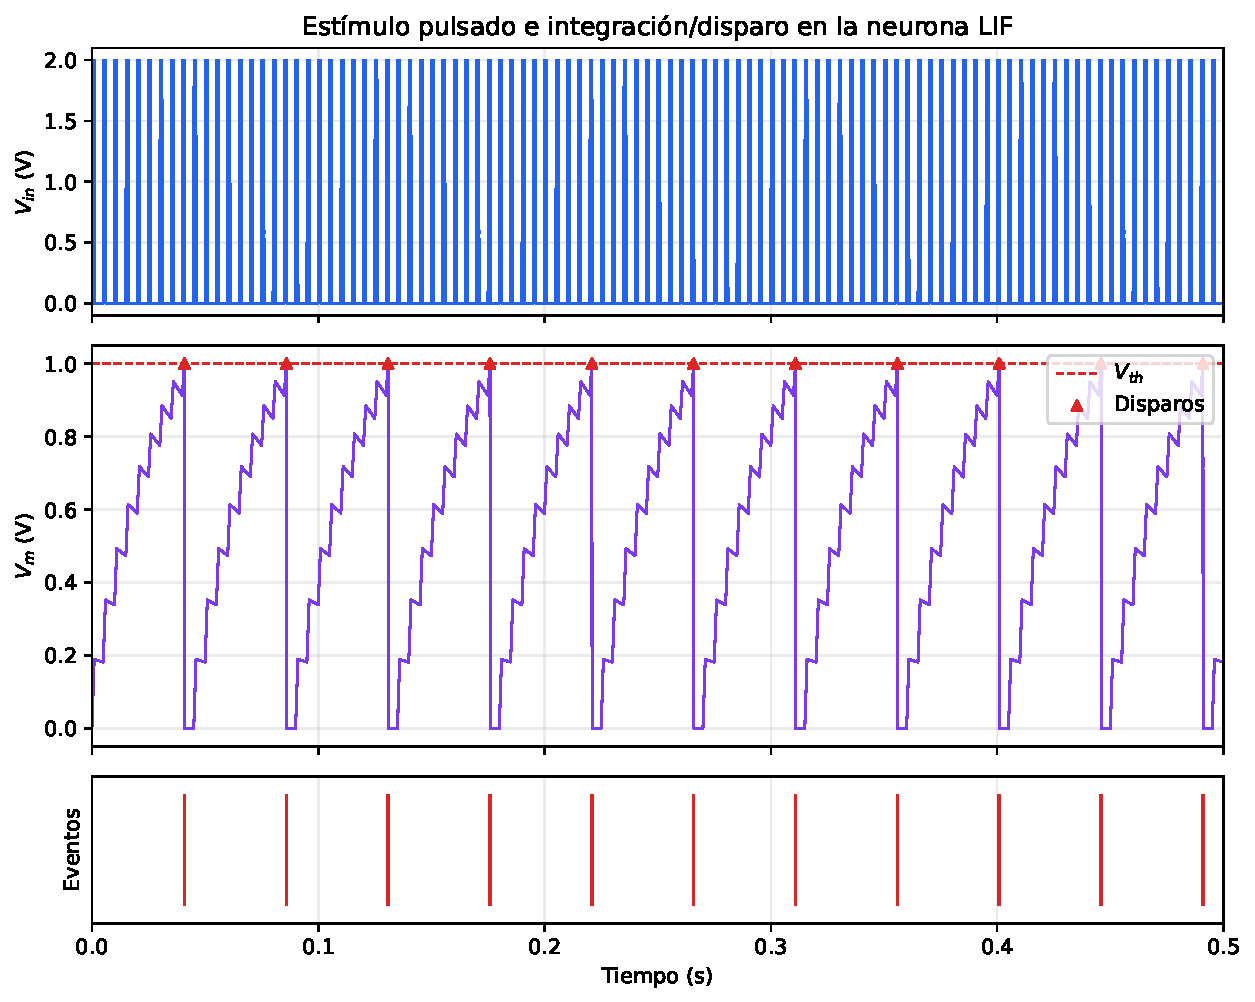
\includegraphics[width=0.95\textwidth]{figuras/fig_13_lif_behavior.pdf}
    \caption[Respuesta de la neurona LIF]{Respuesta de la neurona LIF del simulador: estímulo pulsado, integración del potencial de membrana y eventos de disparo, en concordancia funcional con la dinámica descrita por Wang et al.~\cite{2}.}
    \label{fig:lif-behavior-wang}
\end{figure}

\textbf{Propósito y Relevancia:} La figura documenta que el simulador LIF implementa la secuencia de integración y disparo. El panel inferior es un raster de eventos, no una forma de onda de voltaje de salida ni una medición física.
